\documentclass{article}
\usepackage{amsmath}
\usepackage{amssymb}
\usepackage{ctex}
\usepackage{graphicx}
\begin{document}
\title{��������ҵ}
\maketitle
1.\[\begin{gathered}
  f(x + y) = {c_1}(x + y) + {c_2}(x + y) = {c_1}x + {c_2}x + {c_1}y + {c_2}y = f(x) + f(y) \hfill \\
  f(kx) = {c_1}(kx) + {c_2}(kx) = k({c_1}x + {c_2}x) = kf(x) \hfill \\
  {\text{so }}f(x){\text{ is a linear function}} \hfill \\
  {\text{Because all the real functions make up a linear space,so I only need to}} \hfill \\
  {\text{proof that X' is a subspace}}{\text{.}} \hfill \\
  {f_1}(x) + {f_2}(x) = {c_{11}}{x_1} + {c_{21}}{x_2} + {c_{12}}{x_1} + {c_{22}}{x_2} = ({c_{11}} + {c_{12}}){x_1} + ({c_{21}} + {c_{22}}){x_2} = ({f_1} + {f_2})(x) \hfill \\
  k{f_1}(x) = k({c_1}{x_1} + {c_2}{x_2}) = (k{c_1}){x_1} + (k{c_2}){x_2} = (k{f_1})(x) \hfill \\
  x \in {R^2},x = ({x_1},{x_2}),{\text{denotes the basis as }}{{\text{g}}_1}(x),{g_2}(x) \hfill \\
  \left\{ \begin{gathered}
  {g_1}(x) = {x_1} \hfill \\
  {g_2}(x) = {x_2} \hfill \\
\end{gathered}  \right.,proof:\forall f(x) \in X',f(x) = {c_1}{x_1} + {c_2}{x_2} = {c_1}{g_1}(x) + {c_2}{g_2}(x) \hfill \\
  {k_1}({x_1},0) + {k_2}(0,{x_2}) = 0 \hfill \\
   \Rightarrow ({k_1}{x_1},{k_2}{x_2}) = 0 \hfill \\
   \Rightarrow {k_1} = 0,{k_2} = 0 \hfill \\
  {\text{so }}{g_1}(x){\text{ and }}{g_2}(x){\text{ is a basis of X'}} \hfill \\
\end{gathered} \]
2.\[\begin{gathered}
  f({h_1} + {h_2}) = ({h_1} + {h_2})({s_1}) = {h_1}({s_1}) + {h_2}({s_1}) \hfill \\
  f(kh) = (kh)({s_1}) = kh({s_1}) = kf(h) \hfill \\
  {\text{so }}f(h) = h({s_1}){\text{ is a linear function}} \hfill \\
\end{gathered} \]
3.\begin{figure}[!h]
  \centering
  % Requires \usepackage{graphicx}
  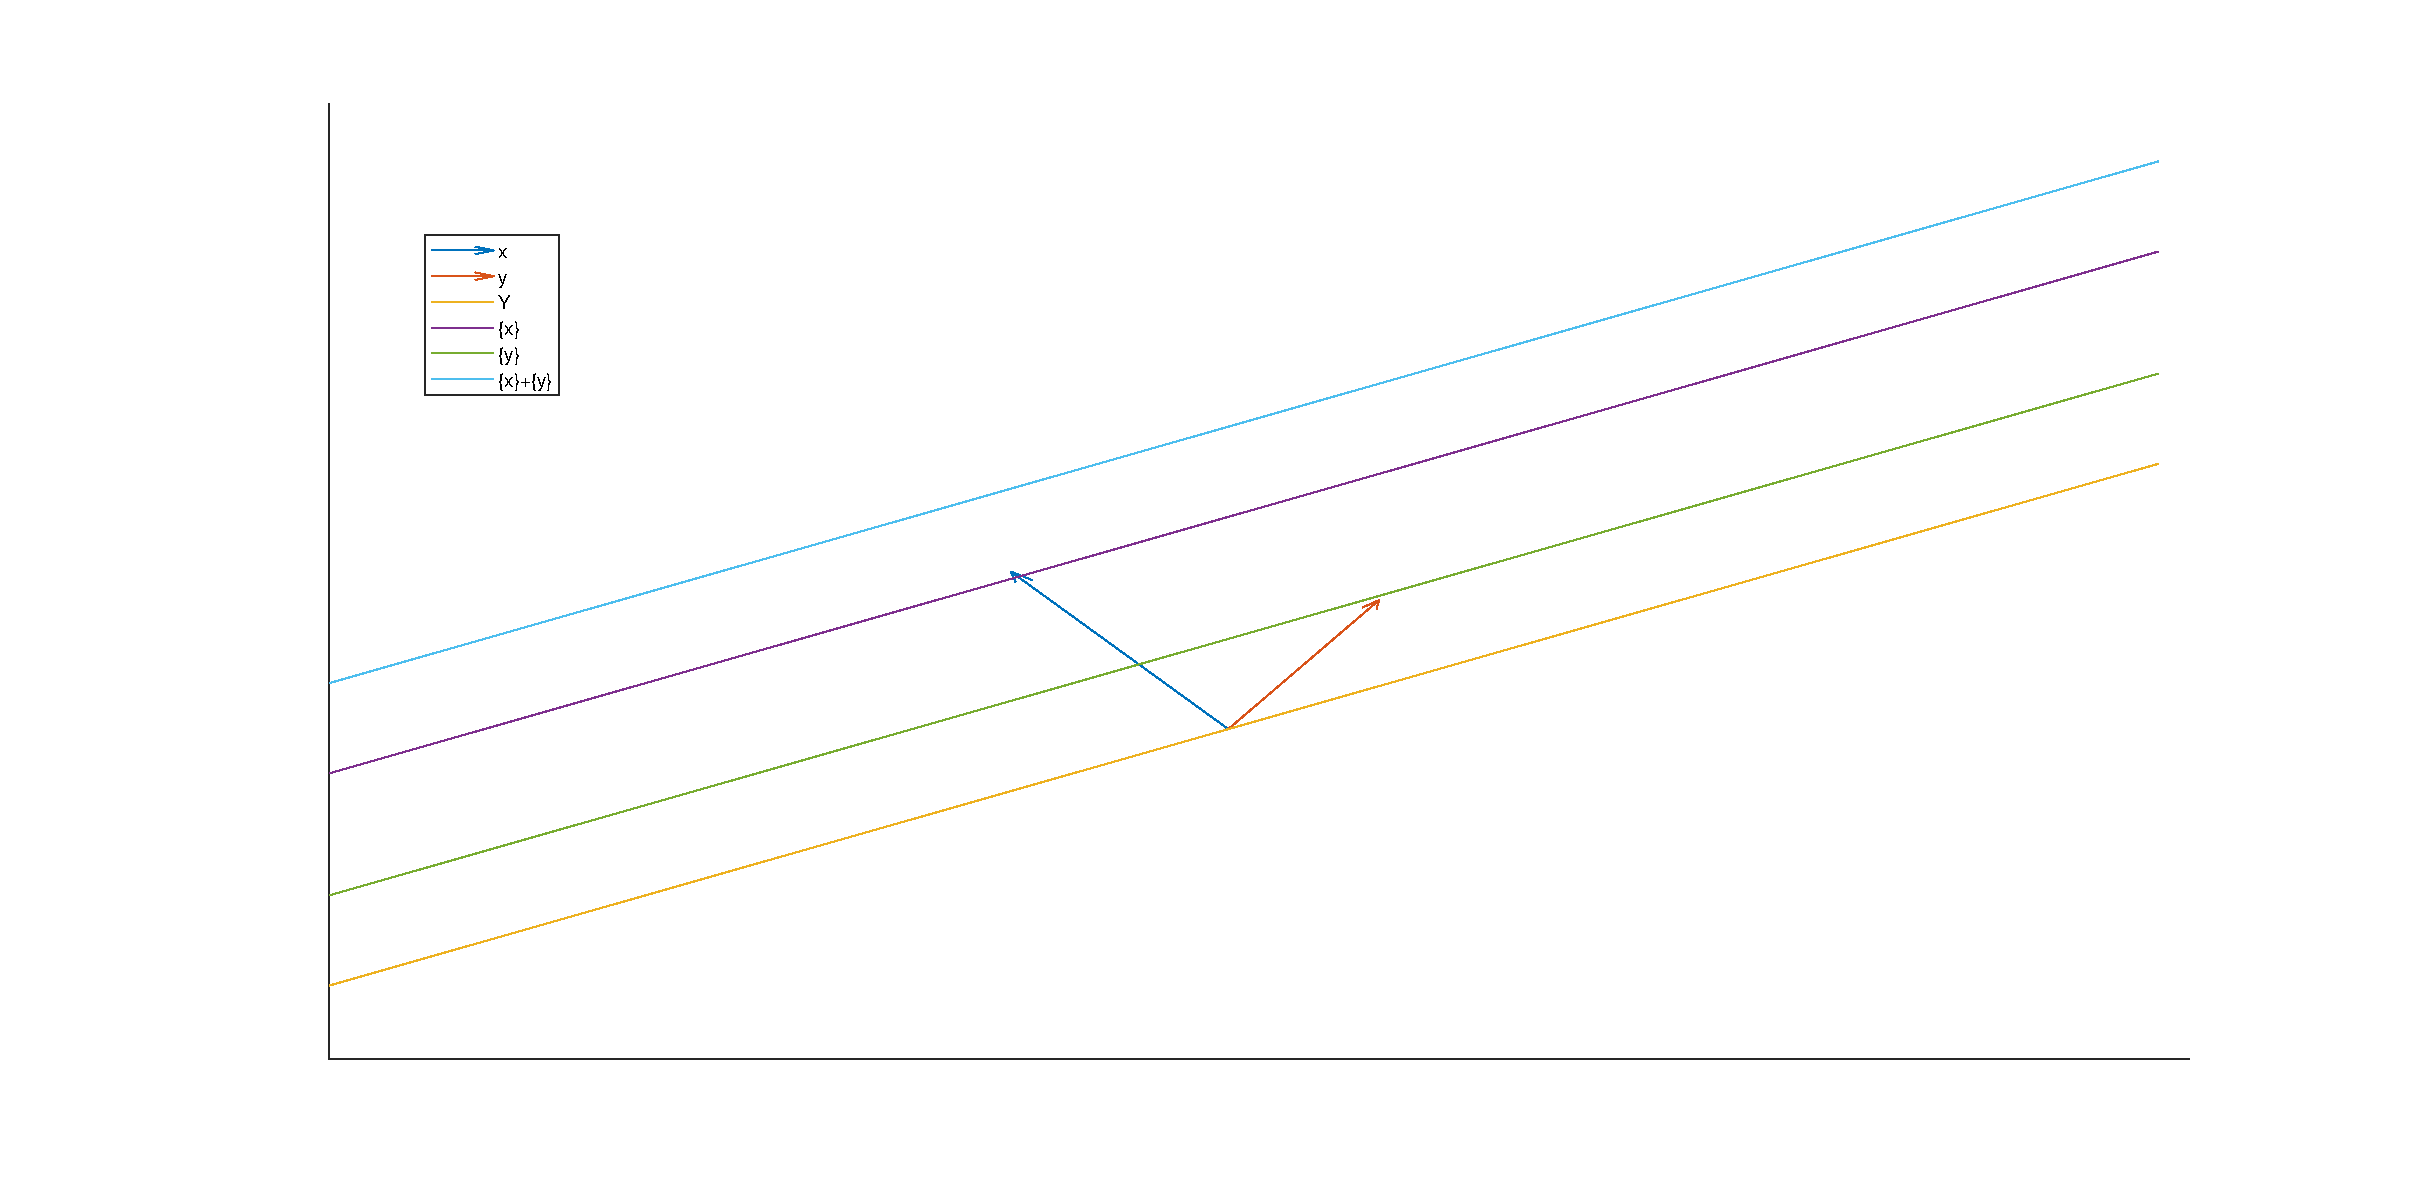
\includegraphics[scale=0.35]{7.eps}\\
  \caption{\{x\},\{y\},\{x+y\}}
\end{figure}
\end{document}
